\topic{Isomorphic Binary Structures}

Consider \(S = \{a, b, c\}, S' = \{1, 2, 3\}\) and binary operations \(*, *'\), defined as the following.
\[
    \begin{array}{c|ccc}
        * & a & b & c \\ \hline
        a & b & a & c \\
        b & c & a & b \\
        c & a & b & c
    \end{array}
    \qquad
    \begin{array}{c|ccc}
        *' & 1 & 2 & 3 \\ \hline
        1  & 2 & 1 & 3 \\
        2  & 3 & 1 & 2 \\
        3  & 1 & 2 & 3
    \end{array}
\]
We see that if we rename \(a, b, c\) to \(1, 2, 3\) respectively, we see that the tables are actually \textit{equivalent}. How do we formalize the notion of equivalence of binary structures \((S, *), (S', *')\)?

\defn. \note{Isomorphism} Let \((S, *)\) and \((S', *')\) be binary structures. If there exists a bijection \(\varphi: S \ra S'\) such that
\begin{center}
    \(\varphi(a * b) = \varphi(a) *' \varphi(b)\), \quad \(\forall a, b \in S\),
\end{center}
then \(\varphi\) is called an \textbf{isomorphism} between \((S, *)\) and \((S', *')\). We say that \((S, *)\) and \((S', *')\) are \textbf{isomorphic} to each other.

\defn. \note{Homomorphism} Let \((S, *)\) and \((S', *')\) be binary structures. A map \(\varphi: S \ra S'\) such that
\begin{center}
    \(\varphi(a * b) = \varphi(a) *' \varphi(b)\), \quad \(\forall a, b \in S\)
\end{center}
is called a \textbf{homomorphism} between \((S, *)\) and \((S', *')\).

\rmk Isomorphisms are \textit{renaming functions} that preserve the structure of a set. Isomorphisms are homomorphisms that are bijective. Also, homomorphisms can be seen as a somewhat confusing(?) renaming functions, since they aren't bijective.

\begin{center}
    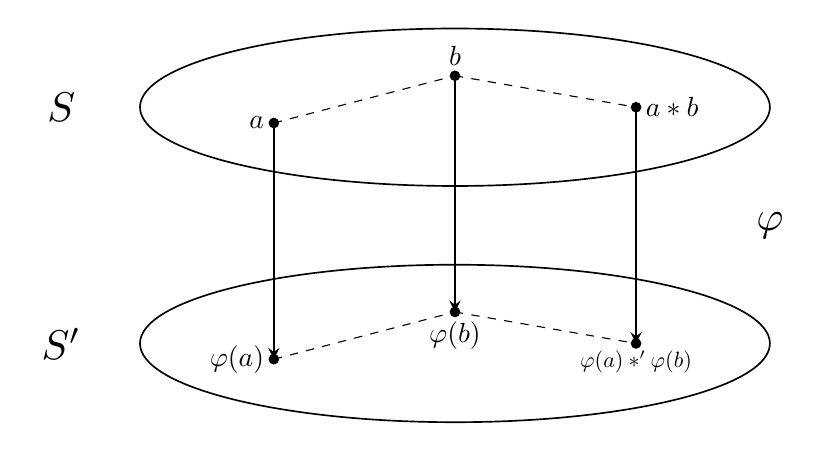
\begin{tikzpicture}
        \draw[semithick] (0, 0) ellipse (4 and 1);
        \draw[semithick] (0, -3) ellipse (4 and 1);

        \coordinate (A) at (-2.3, -0.2);
        \coordinate (B) at (0, 0.4);
        \coordinate (C) at (2.3, 0);

        \coordinate (AA) at (-2.3, -0.2 - 3);
        \coordinate (BB) at (0, 0.4 - 3);
        \coordinate (CC) at (2.3, 0 - 3);

        \filldraw (A) circle (0.06);
        \filldraw (B) circle (0.06);
        \filldraw (C) circle (0.06);

        \filldraw (AA) circle (0.06);
        \filldraw (BB) circle (0.06);
        \filldraw (CC) circle (0.06);

        \draw[-stealth, thick] (A) -- (AA);
        \draw[-stealth, thick] (B) -- (BB);
        \draw[-stealth, thick] (C) -- (CC);

        \draw[dashed] (A) -- (B);
        \draw[dashed] (B) -- (C);

        \draw[dashed] (AA) -- (BB);
        \draw[dashed] (BB) -- (CC);

        \node[scale=1.5] at (4, -1.5) {\(\varphi\)};
        \node[left] at (A) {\(a\)};
        \node[above] at (B) {\(b\)};
        \node[right] at (C) {\(a * b\)};

        \node[left] at (AA) {\(\varphi(a)\)};
        \node[below] at (BB) {\(\varphi(b)\)};
        \node[below, scale=0.8] at (CC) {\(\varphi(a) *' \varphi(b)\)};

        \node[scale=1.5] at (-5, 0) {\(S\)};
        \node[scale=1.5] at (-5, -3) {\(S'\)};

    \end{tikzpicture}
\end{center}

\ex. Examples of isomorphisms.
\begin{enumerate}
    \item Let \(\varphi: (\R, +) \ra (\R^+, \cdot)\) with \(\varphi(x) = e^x\) for \(x \in \R\).
    \item Let \(\varphi: (\Z, +) \ra (2\Z, +)\) with \(\varphi(n) = 2n\) for \(n \in \Z\).
    \item Non-example: \((\Z, *) \not\simeq (\R, *)\) (different cardinality)
\end{enumerate}

\rmk \textbf{Structural properties}: properties preserved by isomorphisms
\begin{enumerate}
    \item Number of elements (cardinality, for infinite sets)
    \item Commutativity, associativity
    \item The equation \(a * x = b\), \(\forall a, b \in S\) has a solution in \(S\)
\end{enumerate}
We can disprove the existence of an isomorphism by showing that any of the structural properties do not hold.

\ex. For \((\Z, \cdot)\) and \((\Z^+, \cdot)\) we want to show that these two are not isomoprhic. Consider the equation \(x^2 = x\). In \(\Z\), the solutions are \(x = 0, 1\), but in \(\Z^+\), the solution is unique, \(x = 1\).

\pf Suppose that \(\Z\) and \(\Z^+\) are isomorphic, and let \(\varphi\) be the isomorphism. Let \(\varphi(0) = a\), \(\varphi(1) = b\). Then \(a \neq b\), since \(\varphi\) is a bijection. However,
\[
    a = \varphi(0 \cdot 0) = \varphi(0) \cdot \varphi(0) = a \cdot a, \quad
    b = \varphi(1 \cdot 1) = \varphi(1) \cdot \varphi(1) = b \cdot b
\]
but in \(\Z^+\) there is only one solution to \(x^2 = x\). This is a contradiction, so \(\varphi\) is not an isomorphism. \qed

\defn. \note{Identity} Let \((S, *)\) be a binary structure. If \(e \in S\) satisfies
\begin{center}
    \(e * a = a * e = a\), \quad \(\forall a \in S\),
\end{center}
then \(e\) is called the \textbf{identity} element of \(S\).

\thm. Identities are unique, if it exists.

\pf Let \(e, e' \in S\) be identities of \(S\). Then, \(e = e * e' = e' * e = e'\) so \(e = e'\). \qed

\thm. If \(\varphi: S \ra S'\) is an isomorphism, \(\varphi\) maps the identity to the identity.

\pf Let \(e \in S\) be the identity of \(S\). For any \(t \in S'\), there exists \(s \in S\) such that \(\varphi(s) = t\). Then
\[
    t *' \varphi(e) = \varphi(s * e) = \varphi(s) = t, \quad
    \varphi(e) *' t = \varphi(e * s) = \varphi(s) = t,
\]
so \(\varphi(e)\) is the identity of \(S'\). \qed

\pagebreak
